This section will explore accepted ways to profile the speed of python applications.
Microsoft Visual Studio recognizes three forms of profiling: sampling, instrumentation, and
tracing\cite{MicrosoftProfiling}.
Profiling is a balance, as the more detailed the profiling, the more overhead is introduced to the script, in this
section we will explore we will explore all the aforementioned methods of profiling, and find the most appropriate
balance between detail and overhead.

\subsubsection{Bash Time}\label{subsubsec:bash_time}
Assuming the script is being run in a bash terminal, the time command\cite{BashTime} is a standard
simple approach to finding execution time; as per the documentation this outputs 3 values: real, user, and sys time.
This is immediately more useful than a regular clock approach, as it gives us insight into the execution time at
different levels of processing.
The bash time function returns results in milliseconds, with both user and sys time being translated from clock ticks
within the CPU - this makes it difficult to judge the accuracy of such measurements, as they are heavily hardware
dependant, for the purpose of this report we will assume it is sufficient.
Lastly, as the timer is not connected to the script being tested, there is no way to create a profiler that can locate
exact points of inefficiency, simply indicate that they exist - this can be partially circumvented by creating
profiles for units of code that can be applied using static profilers.

\begin{figure}[H]
    \centering
    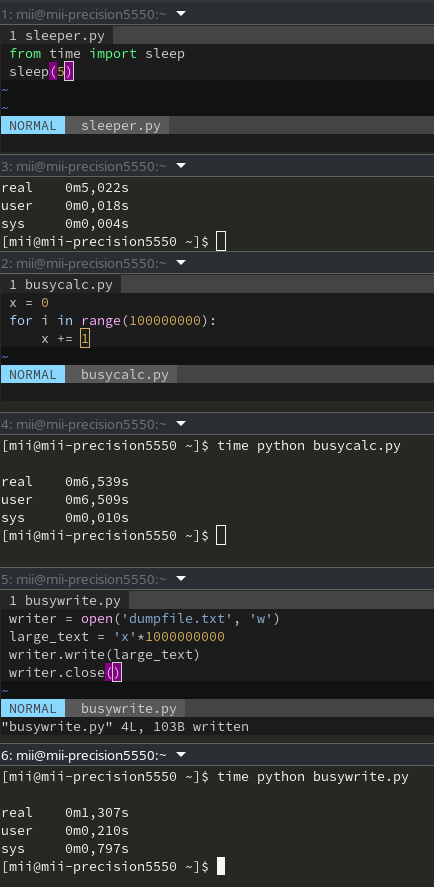
\includegraphics[width=8cm]{figures/introduction/bashtime}
    \caption{Three examples of python scripts being run in bash with time, each script maximises a different aspect of
    time - a sleep will increase overall time without increasing user or sys time; a CPU bound script will increase user
    time; and a script that waits for IO will increase sys time.}
    \label{fig:bash_time}
\end{figure}

\subsubsection{Perf}
Perf is a complex Linux tool designed to collect a myriad of different events, for this section we will focus on the
\textit{record} and \textit{report} functionality, which gathers samples of the \texit{cycles} event, this compiled 
information can be displayed as a report with various different tools, such as the gecko tool displayed in
fig\ref{fig:perf_gecko}.
Perf has the advantage of (if enabled) describing the entire system in its report, unfortunately this requires
additional into threads that may be significant to the execution of the script.

\begin{figure}[H]
    \centering
    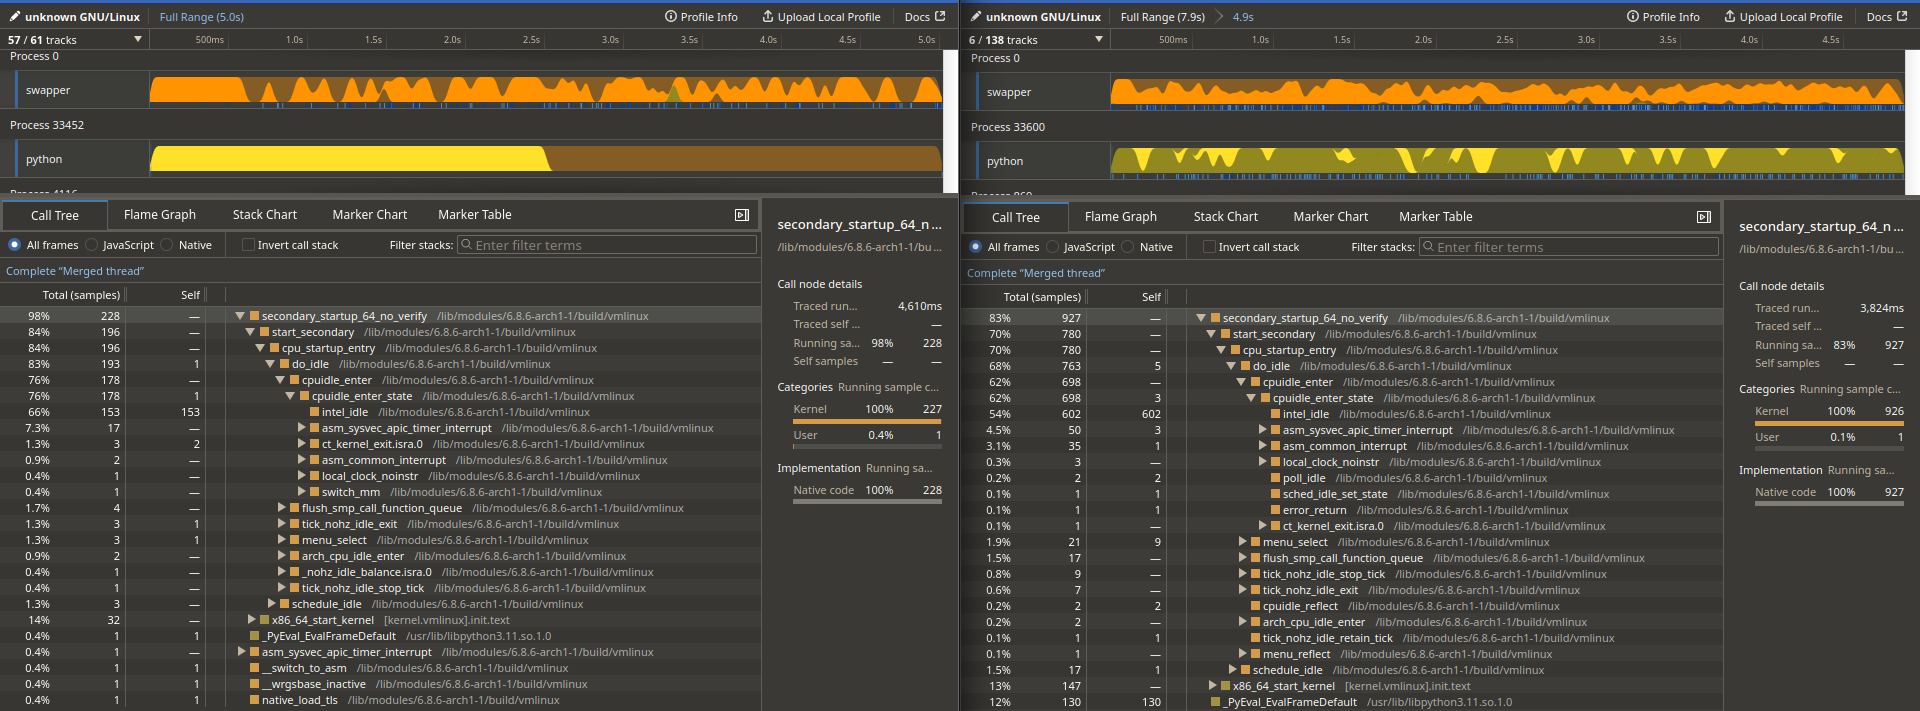
\includegraphics[width=15cm]{figures/introduction/perf_gecko_sleep_vs_calc}
    \caption{Comparing a python script that sleeps for 5 seconds (left) to the busy calc script
    from~\ref{subsubsec:bash_time} (right) note the increased amount of samples for busycalc, which may be used to
    predict its increased load}
    \label{fig:perf_gecko}
\end{figure}

\subsubsection{Python Profiler}
The python profiler\cite{PythonProfiler} is a standard tool for profiling python scripts, it improves on bash time by
providing information on the time within each call of the script, allowing for a more granular understanding of what
might be causing performance bottlenecks.
As per the documentation, the timer is limited by the underlying clock rate (1ms) - additionally due to the time between
an event and the call for the clock state can introduce inaccuracies for calls that execute many times in a short
period.
The python profiler is split into two parts, the cProfile and profile modules, the cProfile module is a C extension with
minimal overhead that is intended for our use-case, while the profile module is a pure python implementation that is
designed to be more approachable for tasks such as creating extensions - for our purposes we will focus on cProfile.
While the python profiler is a powerful tool, it is not without drawbacks, as calls themselves can be nebulous, FIGURE
shows how the previously created \textit(busycalc) script has no definable metrics to explain its time cost,
furthermore, calling \textit(busycalc) with the profiler inexplicably adds 2 seconds of overhead to the execution time
- this is likely due to underlying functionality in Python's approach to garbage collection, and would have to be
investigated if we were to use the profiler as an approach for energy prediction.



\subsubsection{Python Logging}
The most simple method to find execution time is to simply time the execution of a script, either by noting the time
before and after the running of the script, or by logging the time within the script.
The previous sections showed that there are many easy ways to record the time before and after script
execution, so this section will rather focus on situations where this is not desired - namely in applications that are
not expected to run for short periods of time.

Logging is a standard concept within programming, generally used to extrapolate
information about the state of a program from a user's perspective.
The standard python logger\cite{PythonLogging} is simple and allows timings to be attached to log messages, however
this only operates up to a millisecond resolution, so for more precise calculations, this functionality has to be
expanded on.
When logging events, the desired effect is to retrieve the most accurate and high resolution time available, this is
done by running the python in-built time\cite{PythonTime} utility - as of Python3.7, time provides six different
functions at nanosecond resolution\cite{PythonTimePEP}, preventing loss of precision due to floating point calculations.
Similarly to bash time, the different functions provide different insights into the execution of the script, these
can be explored provided that logging is explored as a method of profiling.

The issue with logging is that it is not a standard method of profiling, and requires invasive changes to the script to
provide valuable insights into where time is being invested in the script.
Lastly, as logging is an invasive process, it will undoubtedly affect the performance of the script, which introduces
the decision of correct logging intervals to minimize overhead while still retrieving sufficiently precise data.

\begin{figure}[H]
    \centering
    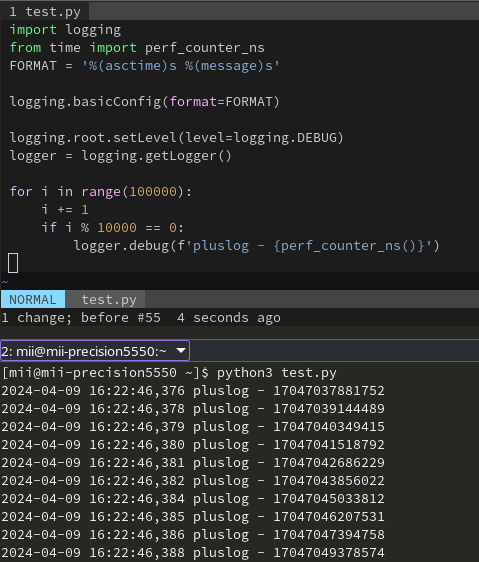
\includegraphics[width=8cm]{figures/introduction/python_log_time}
    \caption{An example of logging being used to find the time after every 10,000 executions of adding to x. Note that
    while the logging library has a time function, there is no way inject higher resolution timers without manually
    calling them. In the output there is also the perf counter, showing a far higher precision output of execution}
    \label{fig:python_log_time}
\end{figure}

\subsubsection{PyTracer}\label{subsubsec:pytracer}
As an alternative to logging, the python sys package includes a settrace module\cite{PythonSystrace} that allows for the
injection of code into individual callbacks of the python interpreter.
This is a powerful tool, as it allows us to analyse individual stack frames, we can use this to analyse executed opcodes
and derive energy usage metrics from predictions of their energy footprint - to understand the opcodes we will need
to make further use of the Disassembler module \textit{dis}\cite{PythonDis}.
Furthermore, these frames contain contextual information that will allow a working profiler to pinpoint areas of
contention to developers.

The major drawback of tracing is similar to logging, as any form of tracing is invasive, and will skew results, this can
be mitigated if the footprint of the tracer is known and accounted for in the final results.

\begin{figure}[H]
    \centering
    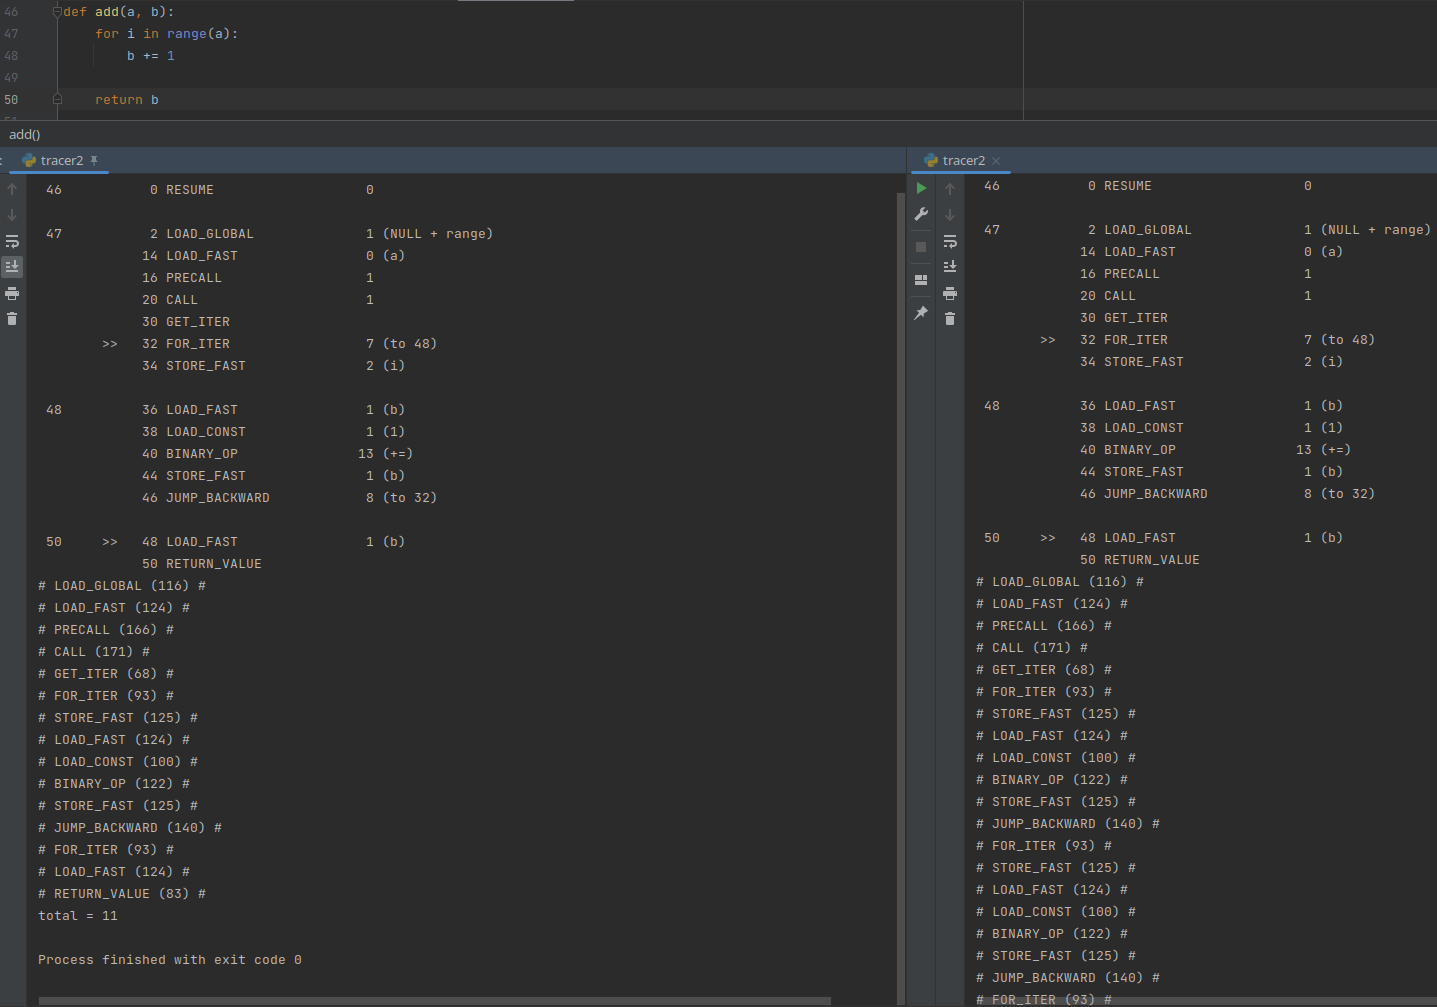
\includegraphics[width=12cm]{figures/introduction/tracer_example}
    \caption{An example of using pytracer to trace the execution of a function that adds two values via iterating over
    the first, the output at the bottom is split into calling \texit{add(1, 10)} (left) and \textit{add(2, 10)} (right),
    first the bytecode of the function is printed using the diassembler module (with line numbers on the far left),
        followed by the individual opcodes being run - note that the output on the right is identical except for the
    repeated opcodes in the output on the right.}
    \label{fig:pytracer_example}
\end{figure}